\documentclass{article}
\usepackage{quiver}
\usepackage{tikz}
\usepackage{tikz-cd}
\usepackage{adjustbox}
\usetikzlibrary{positioning}
\usetikzlibrary{graphs}
\usetikzlibrary{backgrounds}
\usetikzlibrary{arrows.meta}
\newcommand \separator {\bigskip\hrule\bigskip}
\newcommand \hide [1] {\bgroup}
\tikzset{
	mgvertex/.style={
		circle,
		fill,
		inner sep=0pt,
		minimum size=5pt,
		label=#1:{\tikzgraphnodetext},
		execute at begin node=\hide,
		graphs/as={}
	},
	mgvertex/.default={above},
	mg/.style={
		graphs/every graph/.style = {grow right sep = 15mm},
		every edge quotes/.style = {draw,fill=white,sloped,midway,->},
		baseline = (current bounding box.center)
	},
	k1/.pic = {
		\graph {
			0 [mgvertex=left] -!- 1 [mgvertex=right] ;
			2 [mgvertex=left] -!- 3 [mgvertex=right] ;
		} ;
	},
	l1/.pic = {
		\graph {
			0 [mgvertex=left] -> ["a"] 1 [mgvertex=right] ;
			2 [mgvertex=left] -> ["b"] 3 [mgvertex=right] ;
		} ;
	},
	l2/.pic = {
		\graph {
			4 [mgvertex=left] -> ["a"] 5 [mgvertex=right];
		} ;
	},
	k2/.pic = {
		\graph {
			4 [mgvertex=left]-!- 5 [mgvertex=right];
		} ;
	}
}

\begin{document}

Consider these two rewrite rules:

\begin{center}
	\begin{tikzcd}
		R_1 & K_1 & L_1 \\
		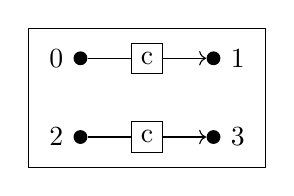
\begin{tikzpicture}[mg,framed]
			\graph {
				0 [mgvertex=left] -> ["c"] 1 [mgvertex=right] ;
				2 [mgvertex=left] -> ["c"] 3 [mgvertex=right] ;
			} ;
		\end{tikzpicture} &
		\tikz[mg,framed]{\pic{k1};} &
		\tikz[mg,framed]{\pic{l1};}
		\arrow[from=2-2,to=2-1]
		\arrow[from=2-2,to=2-3]
	\end{tikzcd}
	
	\begin{tikzcd}
		L_2 & K_2 & R_2 \\
		\tikz[mg,framed] {\pic{l2};} &
		\tikz[mg,framed] {\pic{k2};} &
		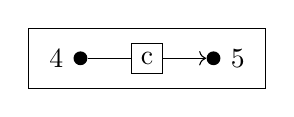
\begin{tikzpicture}[mg,framed]
			\graph {
				4 [mgvertex=left] -> ["c"] 5 [mgvertex=right];
			} ;
		\end{tikzpicture}
		\arrow[from=2-2,to=2-1]
		\arrow[from=2-2,to=2-3]
	\end{tikzcd}
\end{center}

In order to compute its critical pairs, we first start by computing the product hypergraph $L_1 \times L_2$,

\begin{center}
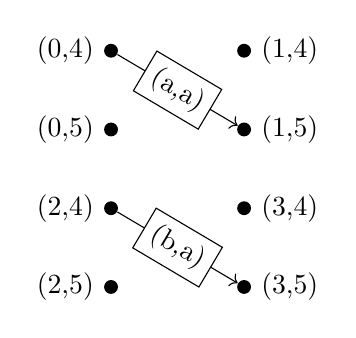
\begin{tikzpicture} [mg] 
	\graph {
		04/{(0,4)} [mgvertex=left] -!- 14/{(1,4)} [mgvertex=right] ;
		05/{(0,5)} [mgvertex=left] -!- 15/{(1,5)} [mgvertex=right] ;
		24/{(2,4)} [mgvertex=left] -!- 34/{(3,4)} [mgvertex=right] ;
		25/{(2,5)} [mgvertex=left] -!- 35/{(3,5)} [mgvertex=right] ;

		04 -> ["(a,a)"] 15 ;
		24 -> ["(b,a)"] 35
	} ;
\end{tikzpicture}
\end{center}

\noindent and then filtering out incompatible pairs of edges.

\begin{center}
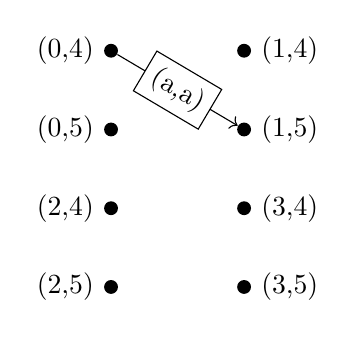
\begin{tikzpicture} [mg]
	\graph {
		04/{(0,4)} [mgvertex=left] -!- 14/{(1,4)} [mgvertex=right] ;
		05/{(0,5)} [mgvertex=left] -!- 15/{(1,5)} [mgvertex=right] ;
		24/{(2,4)} [mgvertex=left] -!- 34/{(3,4)} [mgvertex=right] ;
		25/{(2,5)} [mgvertex=left] -!- 35/{(3,5)} [mgvertex=right] ;

		04 -> ["(a,a)"] 15 ;
	} ;
\end{tikzpicture}
\end{center}

Next step is, for every subgraph, to compute its glueing. For example,

\begin{center}
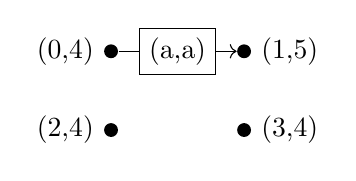
\begin{tikzpicture} [mg] 
	\graph {
		04/{(0,4)} [mgvertex=left] -> ["(a,a)"] 15/{(1,5)} [mgvertex=right] ;
		24/{(2,4)} [mgvertex=left] -!- 34/{(3,4)} [mgvertex=right] ;
	} ;
\end{tikzpicture}
\end{center}

gets us the following:

\begin{center}
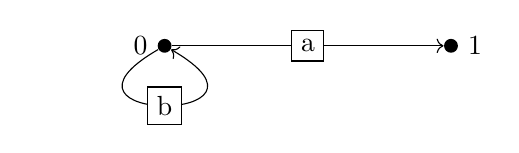
\begin{tikzpicture} [mg]
	\graph {
		0 [mgvertex=left] -> ["a"] 1 [mgvertex=right, right=50pt of 0] ;
		0 -> ["b",controls=+(210:2) and +(330:2)] 0;
	} ;
\end{tikzpicture}
\end{center}

This gluing fails the monogamous acyclic condition and will be discarded. Let's take a look at another gluing which will succeed. The following subgraph~:

\begin{center}
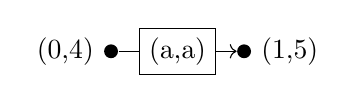
\begin{tikzpicture} [mg] 
	\graph {
		04/{(0,4)} [mgvertex=left] -> ["(a,a)"] 15/{(1,5)} [mgvertex=right] ;	} ;
\end{tikzpicture}
\end{center}

yields the following glued hypergraph~:

\begin{center}
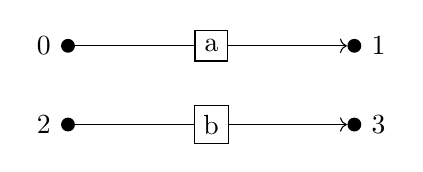
\begin{tikzpicture} [mg]
	\graph {
		0 [mgvertex=left] -> ["a"] 1 [mgvertex=right, right=50pt of 0] ;
		2  [mgvertex=left]  -> ["b"] 3 [mgvertex=right, right=50pt of 0];
	} ;
\end{tikzpicture}
\end{center}

%TODO

Finally, compute the pushout complements and the interface, to yield this:

\bigskip
\begin{adjustbox}{width=\textwidth}
% https://q.uiver.app/#q=WzAsOCxbMCwwLCJLXzEiXSxbMSwwLCJMXzEiXSxbMiwxLCIgQyJdLFszLDAsIkxfMiJdLFs0LDAsIktfMiJdLFs0LDEsIlxcYnVsbGV0Il0sWzAsMSwiXFxidWxsZXQiXSxbMiwyLCJcXGJ1bGxldCJdLFswLDFdLFsxLDJdLFszLDJdLFs0LDNdLFs0LDVdLFs1LDJdLFs2LDJdLFs3LDJdLFs3LDZdLFs3LDVdLFswLDZdLFsyLDQsIiIsMSx7InN0eWxlIjp7Im5hbWUiOiJjb3JuZXIifX1dLFsyLDAsIiIsMSx7InN0eWxlIjp7Im5hbWUiOiJjb3JuZXIifX1dXQ==
$$\begin{tikzcd}
	{\tikz[mg,framed]{\pic{k1};}} &
	{\tikz[mg,framed]{\pic{l1};}} &&
	{\tikz[mg,framed]{\pic{l2};}} &
	{\tikz[mg,framed]{\pic{k2};}} \\
	{\tikz[mg,framed]{\pic{k1};}} &&
	{\tikz[mg,framed]{\graph{
		0 [mgvertex=left] ->["a"] 1 [mgvertex=right];
		2 [mgvertex=left] ->["b"] 3 [mgvertex=right]};}} &&
	{\tikz[mg,framed]{\graph{
		0 [mgvertex=left] -!- 1 [mgvertex=right];
		2 [mgvertex=left] ->["b"] 3 [mgvertex=right]}}} \\
	&& {\tikz[mg,framed]{\pic{k1};}}
	\arrow[from=1-1, to=1-2]
	\arrow[from=1-1, to=2-1]
	\arrow[from=1-2, to=2-3]
	\arrow[from=1-4, to=2-3]
	\arrow[from=1-5, to=1-4]
	\arrow[from=1-5, to=2-5]
	\arrow[from=2-1, to=2-3]
	\arrow["\lrcorner"{anchor=center, pos=0.125, rotate=180}, draw=none, from=2-3, to=1-1]
	\arrow["\lrcorner"{anchor=center, pos=0.125, rotate=90}, draw=none, from=2-3, to=1-5]
	\arrow[from=2-5, to=2-3]
	\arrow[from=3-3, to=2-1]
	\arrow[from=3-3, to=2-3]
	\arrow[from=3-3, to=2-5]
\end{tikzcd}$$
\end{adjustbox}

\end{document}
